%!TEX root = ../../entwurfsprojekt2_entwurfsdokument.tex


\section*{Umgebung}

\begin{figure}
	\centering
	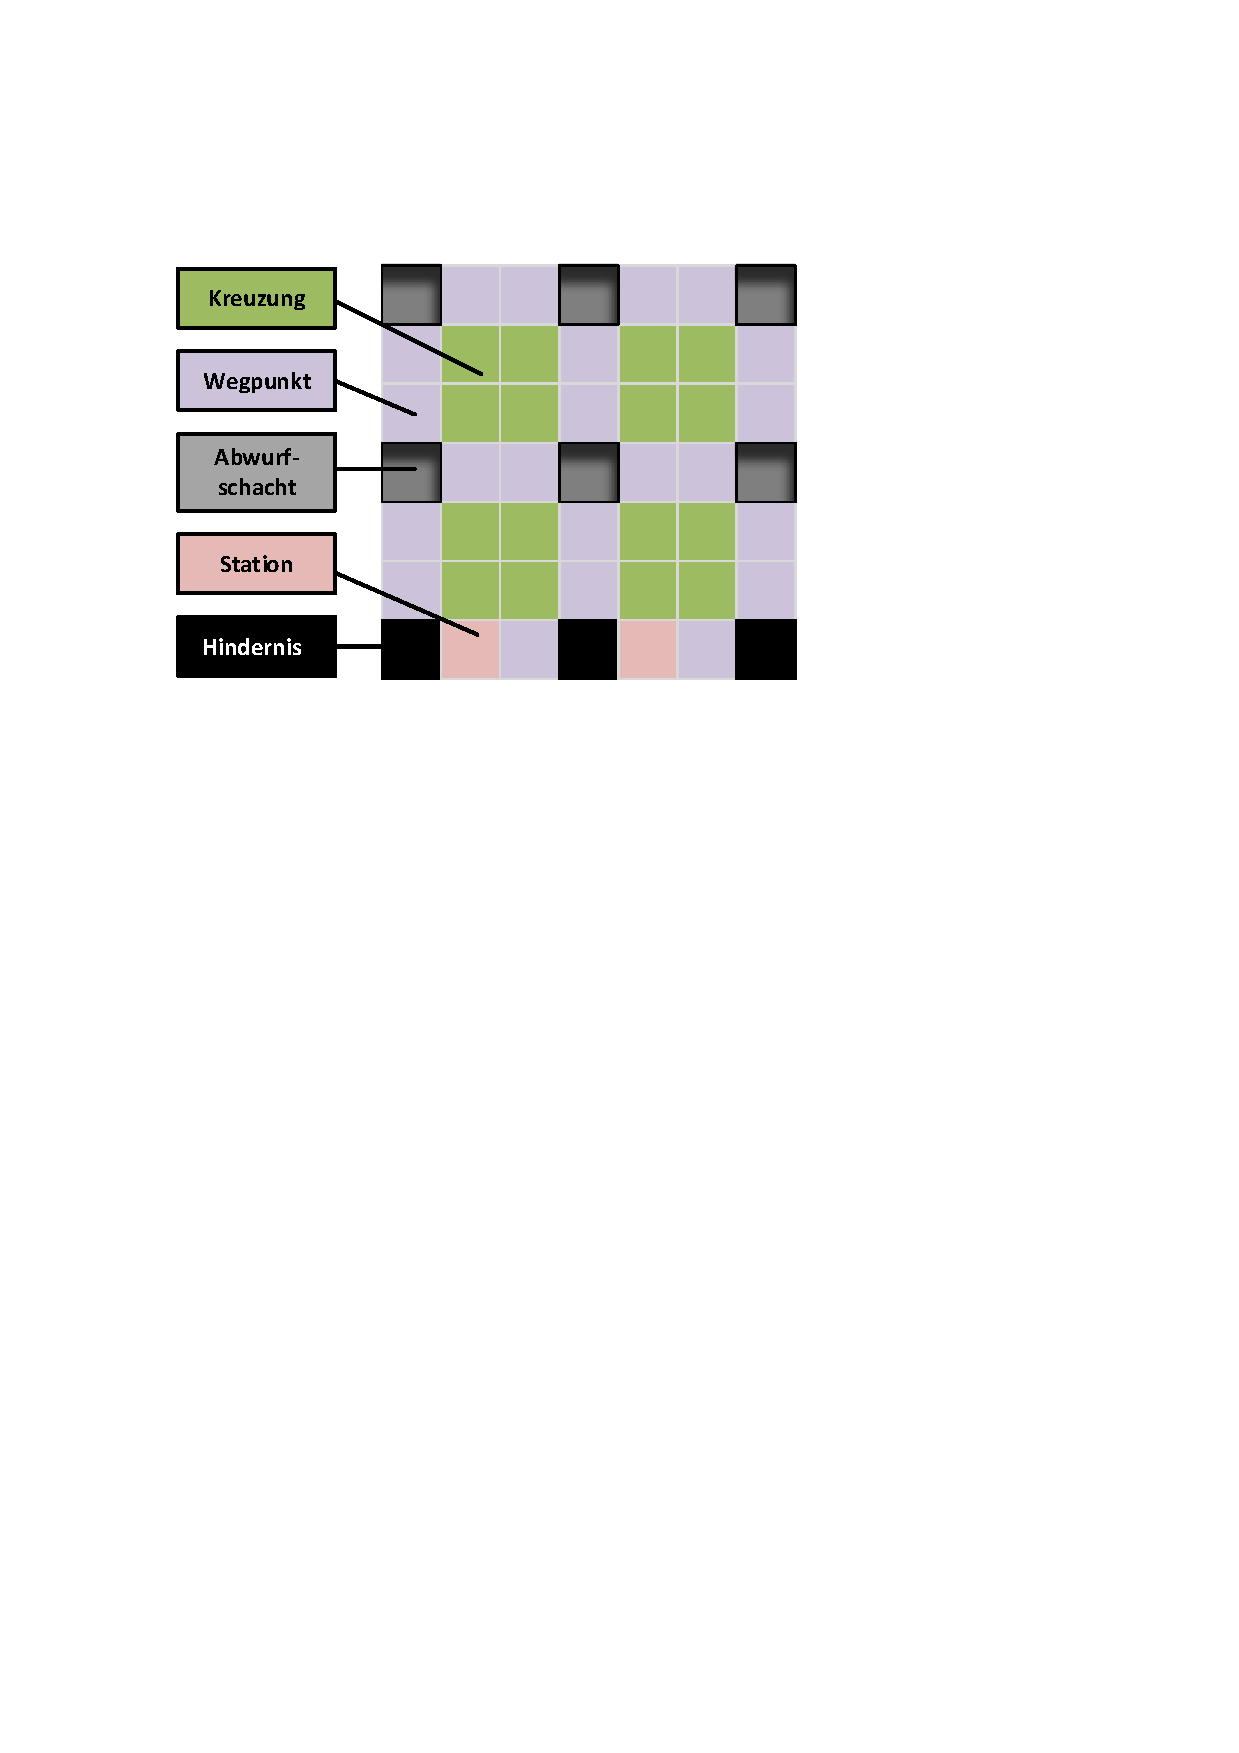
\includegraphics[scale=0.8]{fieldtypes_grid}
	\caption{Übersicht über den Aufbau der Paketsortieranlage und die wichtigsten Begriffe. Die Farben der Felder kennzeichnen die Positionstypen, die von den Robotersensoren erkannt werden können.}
	\label{fig:grid_field_naming}
\end{figure}



\begin{figure}
    \centering
	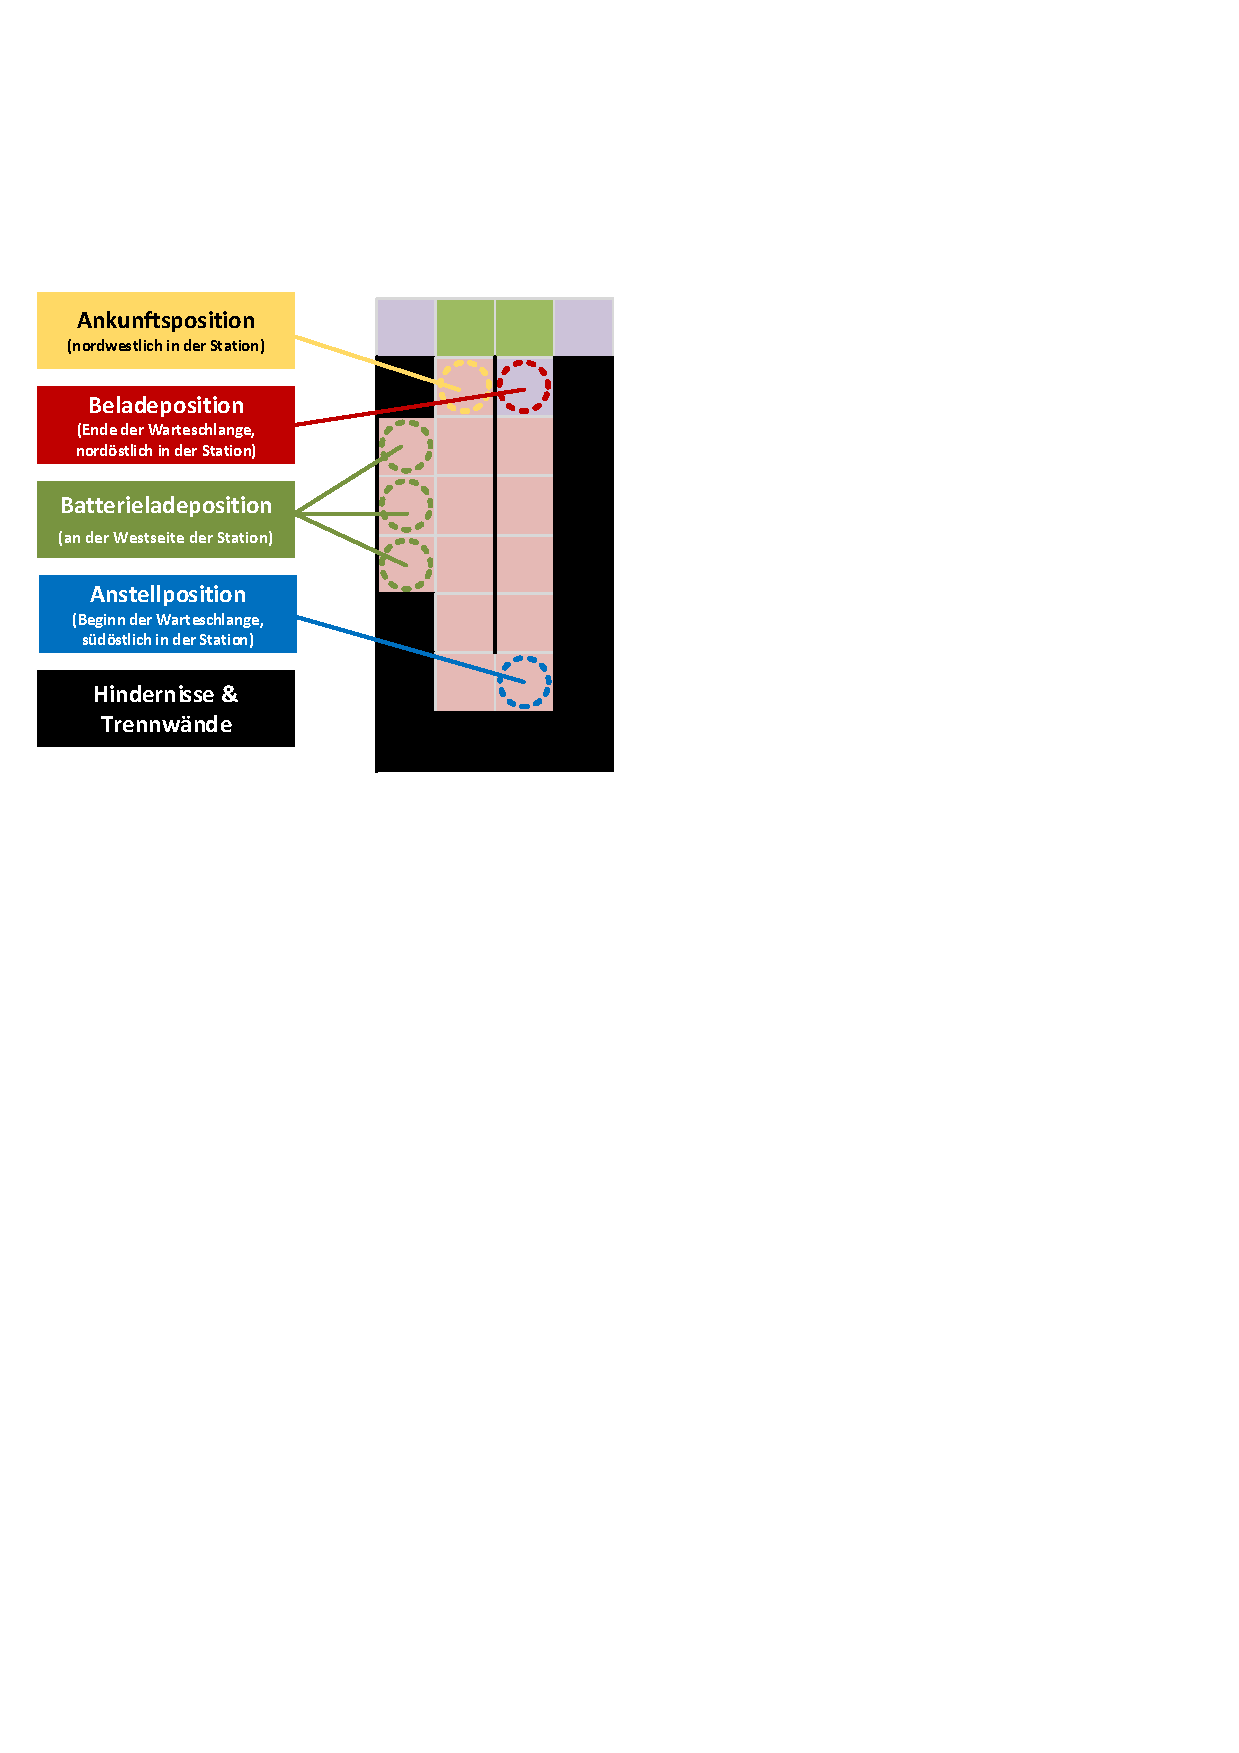
\includegraphics[scale=0.8]{fieldtypes_station}
	\caption{Übersicht über den Aufbau einer Station in der Paketsortieranlage, inklusive der wichtigsten Bezeichnungen für die einzelnen Positionen, zu denen ein Roboter disponiert werden kann.}
	\label{fig:grid_station_naming}
\end{figure}

Die Struktur der Paketsortieranlage ist in \autoref{fig:grid_field_naming} dargestellt und im Folgenden beschrieben. 
Die (potentiell beliebig große) Fläche der Sortieranlage ist in quadratische Felder eingeteilt, die jeweils ganzzahlige Koordinaten haben und gezielt von den Robotern angefahren werden können. 
Die Felder sind jeweils groß genug, so dass ein Roboter sich auf der Stelle drehen kann, ohne mit den Robotern auf den Nachbarfeldern zu kollidieren.

Auf der Fläche der Sortieranlage befinden sich in regelmäßigen Abständen \emph{Abwurfschächte}. 
Zwischen je zwei Abwurfschächten sind immer zwei Felder frei. 
Die Streifen zwischen den Schächten bilden \emph{Straßen}, die aus \emph{Kreuzungen} und sogenannten \emph{Wegpunkten} bestehen.
Auf den Straßen herrscht \textbf{strikter Rechtsverkehr}. 
An Kreuzungen gilt die \textbf{Vorfahrtsregel \enquote{Rechts vor Links}}. 
Durch diese beiden Regeln können autonom fahrende Roboter Kollisionen und Deadlocks vermeiden.

An der Südseite der Sortieranlage befinden sich nebeneinander aufgereiht mehrere \emph{Stationen}, die der in \autoref{fig:grid_station_naming} gezeigten Struktur entsprechen.
Als Übergang zwischen einer Station und der restlichen Fläche der Sortieranlage dienen zwei Felder: die \emph{Ankunftsposition}, auf der rechtsseitig fahrende Roboter aus dem freien Verkehr ankommen, und die \emph{Beladeposition}, von der aus sich Roboter in den Verkehr einordnen können.

Innerhalb einer Station befindet sich links eine Strecke, an der die \emph{Batterieladepositionen} liegen. 
Fährt ein Roboter rückwärts in die Batterieladeposition hinein, beginnt die Aufladung automatisch. 
Die serverseitige Roboterdisposition stellt sicher, dass diese Strecke links der Station immer nur von einem Roboter befahren wird, so dass beim Aus- und Einparken nicht auf Kollisionen geachtet werden muss.

Auf der rechten Seite der Station befindet sich eine \emph{Warteschlange}, in der Roboter darauf warten, beladen zu werden. 
Die vorderste Position der Warteschlange ist die Beladeposition und zugleich der Eintrittspunkt in den regulären Verkehr. 
Da sich die Beladeposition vor einer Kreuzung befindet, erkennt ein darauf stehender Roboter sie als einen Wegpunkt. 
Die Roboter werden zuerst immer zur \emph{Anstellposition} (Ende der Warteschlange) dirigiert und erst danach zur Beladeposition.

Aufgrund von Trennwänden zwischen der rechten und der linken Hälfte der Station, erkennen die Roboter die entsprechenden Nachbarfelder als blockiert. 
Gleiches gilt für \emph{Hindernisse} und Abwurfschächte.

